\chapter{\label{analysis}Аналитический раздел}

В данном разделе будет проведен анализ предметной области, будет проведено сравнение существующих решений. 
Также будет проведена формализация и описание информации, подлежащей хранению в проектируемой базе данных, будут выделены типы пользователей проектируемого приложения к базе данных, а также будет выбрана модель базы данных.

\section{Анализ предметной области}

В данном подразделе будет формально описан список продуктов первой необходимости, будут определены основные типы акций на продукты и основные участники в цепи поставок товаров. Также будет описан <<Меркурий>> --- автоматизированная система для отслеживания продуктов питания на всей цепи их производства и будут формально описаны виды сертификатов на товары.

\subsection{Элементы продуктовой корзины первой необходимости}

Согласно постановлению Правительства № 530 \cite{info_essential_goods2}, элементами продуктовой корзины первой необходимости являются следующие продукты:

\begin{itemize}[label=--]
	\item говядина, баранина, свинина (кроме бескостного мяса);
	\item куры (кроме куриных окорочков);
	\item рыба мороженая неразделанная;
	\item масло сливочное;
	\item масло подсолнечное;
	\item молоко питьевое;
	\item яйца куриные;
	\item сахар-песок;
	\item соль поваренная пищевая;
	\item чай черный байховый;
	\item мука пшеничная;
	\item хлеб ржаной, ржано-пшеничный;
	\item хлеб и булочные изделия из пшеничной муки;
	\item рис шлифованный;
	\item пшено;
	\item крупа гречневая -- ядрица;
	\item вермишель;
	\item картофель;
	\item капуста белокочанная свежая;
	\item лук репчатый;
	\item морковь;
	\item яблоки.
\end{itemize}

\subsection{Акции на товары}

На данный момент рынок розничной торговли очень насыщен. 
С каждым днем среди производителей конкуренция растет высокими темпами. 
Одной рекламы порой бывает не достаточно, чтобы привлечь внимание к производителю и его продукции. 
Чтобы хоть как то выделиться среди многочисленных фирм и предприятий, компаниям необходимо прибегать к методам стимулирования сбыта продукции \cite{info_stock}.

Одна из форм стимулирования --- \textbf{ценовая} \cite{info_stock}. 
Ее суть заключается в установлении скидки на определенный товар или группу товаров.
Можно выделить 5 основных типов акций со снижением  цены \cite{info_promotion1, info_promotion2}:

\begin{itemize}[label*=--]
	\item скидка <<товар дня>>;
	\item скидка за объем, в том числе по принципу <<1+1=3>>;
	\item cкидка отдельным категориям покупателей;
	\item скидка, приуроченная к определенному событию;
	\item сезонная распродажа.
\end{itemize}

\subsection{Цепь поставок}

Предприятия, принимающие участие в создании, распространении и реализации товаров, взаимодействуют в рамках \textbf{цепи поставок}. Они рассматриваются как изолированные элементы, которые самостоятельно планируют свои потребности и покупки с взаимодействуют друг с другом \cite{info_supply_chain}.

Основными участниками цепи поставок являются:

\begin{enumerate}
	\item \textbf{ритейлер} -- организация, которая продает товар конечным потребителям, реализуя его в торговых точках. Ритейлер закупает товар у дистрибьютора;
	\item \textbf{дистрибьютор} -- посредник, который покупает товар у производителя оптовыми партиями для последующей продажи розничным продавцам;
	\item \textbf{производитель} -- организация, создающая товары или услуги, используя сырьевые материалы и компоненты, а также отвечающая за первоначальное распределение продукции.
\end{enumerate}

\subsection{ФГИС <<Меркурий>>}

\textbf{ФГИС <<Меркурий>>} --- автоматизированная система, предназначенная для отслеживания продуктов питания на всей цепи производства и перемещения до точки реализации \cite{info_mercury}.
Работа с <<Меркурием>> заключается в создании и <<гашении>> \textbf{ветеринарно-сопроводительных документов (ВСД)} на всех этапах движения товара: от производства и переработки до продажи или утилизации.

Создание ФГИС <<Меркурий>> позволило достичь следующих целей \cite{info_mercury2}:

\begin{itemize}[label=--]
	\item защита потребителя от некачественной и небезопасной продукции, а все население страны от экономических и социальных угроз;
	\item обеспечение прозрачности и эффективности действий надзорных органов в борьбе с мошенничеством;
	\item минимизация бюрократии и предоставление удобного прозрачного механизма для комфортной работы частного бизнеса.
\end{itemize}

Помимо ВСД существует еще 3 типа разрешительных документов на пищевую продукцию \cite{info_certificates}: 

\begin{itemize}[label*=--]
	\item декларация о соответствии на пищевую продукцию (ДС);
	\item добровольный сертификат на пищевую продукцию;
	\item свидетельство о государственной регистрации пищевой продукции (СГР на пищевую продукцию).
\end{itemize}

\clearpage

\section{Существующие решения}

На рынке существует большое количество сервисов для мониторинга цен на продукты в различных магазинах. Наиболее популярными являются:

\begin{itemize}[label=--]
	\item <<Едадил>> \cite{info_edadil};
	\item SkidkaOnline \cite{info_skidka_online};
	\item Price.ru \cite{info_price_ru}.
\end{itemize}

Сравнение существующих решений было произведено в таблице \ref{tbl:exist_sol}:

\begin{table}[!h]
	\begin{center}
		\begin{threeparttable}
			\caption{Сравнение существующих решений}
			\label{tbl:exist_sol}
			\begin{tabular}{|p{7cm}|c|c|c|}
				\hline
				\textbf{Критерии} & <<Едадил>> & SkidkaOnline & Price.ru \\
				\hline
				возможность сравнения цены на конкретный товар в разных магазинах & + & - & + \\
				\hline
				возможность оставить отзыв о товаре & + & + & + \\
				\hline
				наличие информации об акциях на товары & + & + & + \\
				\hline
				возможность просмотра сертификатов соответствия конкретного товара & - & - & - \\
				\hline
			\end{tabular}
		\end{threeparttable}			
	\end{center}
\end{table}

\clearpage 

\section{Формализация и описание информации, подлежащей хранению в проектируемой базе данных}

На основе анализа предметной области, в разрабатываемой базе данных были выделены сущности, приведенные в таблице \ref{tbl:db_entities}: 

\begin{table}[!h]
	\begin{center}
		\begin{threeparttable}
			\caption{Выделенные сущности предметной области и их описание}
			\label{tbl:db_entities}
			\begin{tabular}{|p{4.5cm}|p{10cm}|}
				\hline
				\textbf{Сущность} & \textbf{Сведения} \\ \hline
				Пользователь & ФИО, номер телефона, пароль, дата регистрации \\ 
				\hline
				Магазин & Название, телефон, адрес, ФИО директора \\ 
				\hline
				Товар & Название, категория, бренд, состав, масса брутто, масса нетто, тип упаковки \\ 
				\hline
				Сертификат соответствия & Тип сертификата, номер сертификата, нормативный документ, дата регистрации сертификата, дата окончания действия сертификата, статус соответствия \\ 
				\hline
				Акция & Тип акции, дата начала, дата конца, размер скидки, описание \\ 
				\hline
				Оценка товара & Отзыв, рейтинг \\ 
				\hline
				Производитель & Название, адрес, номер телефона, ФИО представителя \\ 
				\hline
				Дистрибьютор & Название, адрес, номер телефона, ФИО представителя \\ 
				\hline
				Ритейлер & Название, адрес, номер телефона, ФИО представителя \\ 
				\hline
			\end{tabular}
		\end{threeparttable}
	\end{center}
\end{table}

\clearpage

На рисунке \ref{img:er-diag.drawio.pdf} представлена ER-диаграмма сущностей проектируемой базы данных в нотации Чена:

%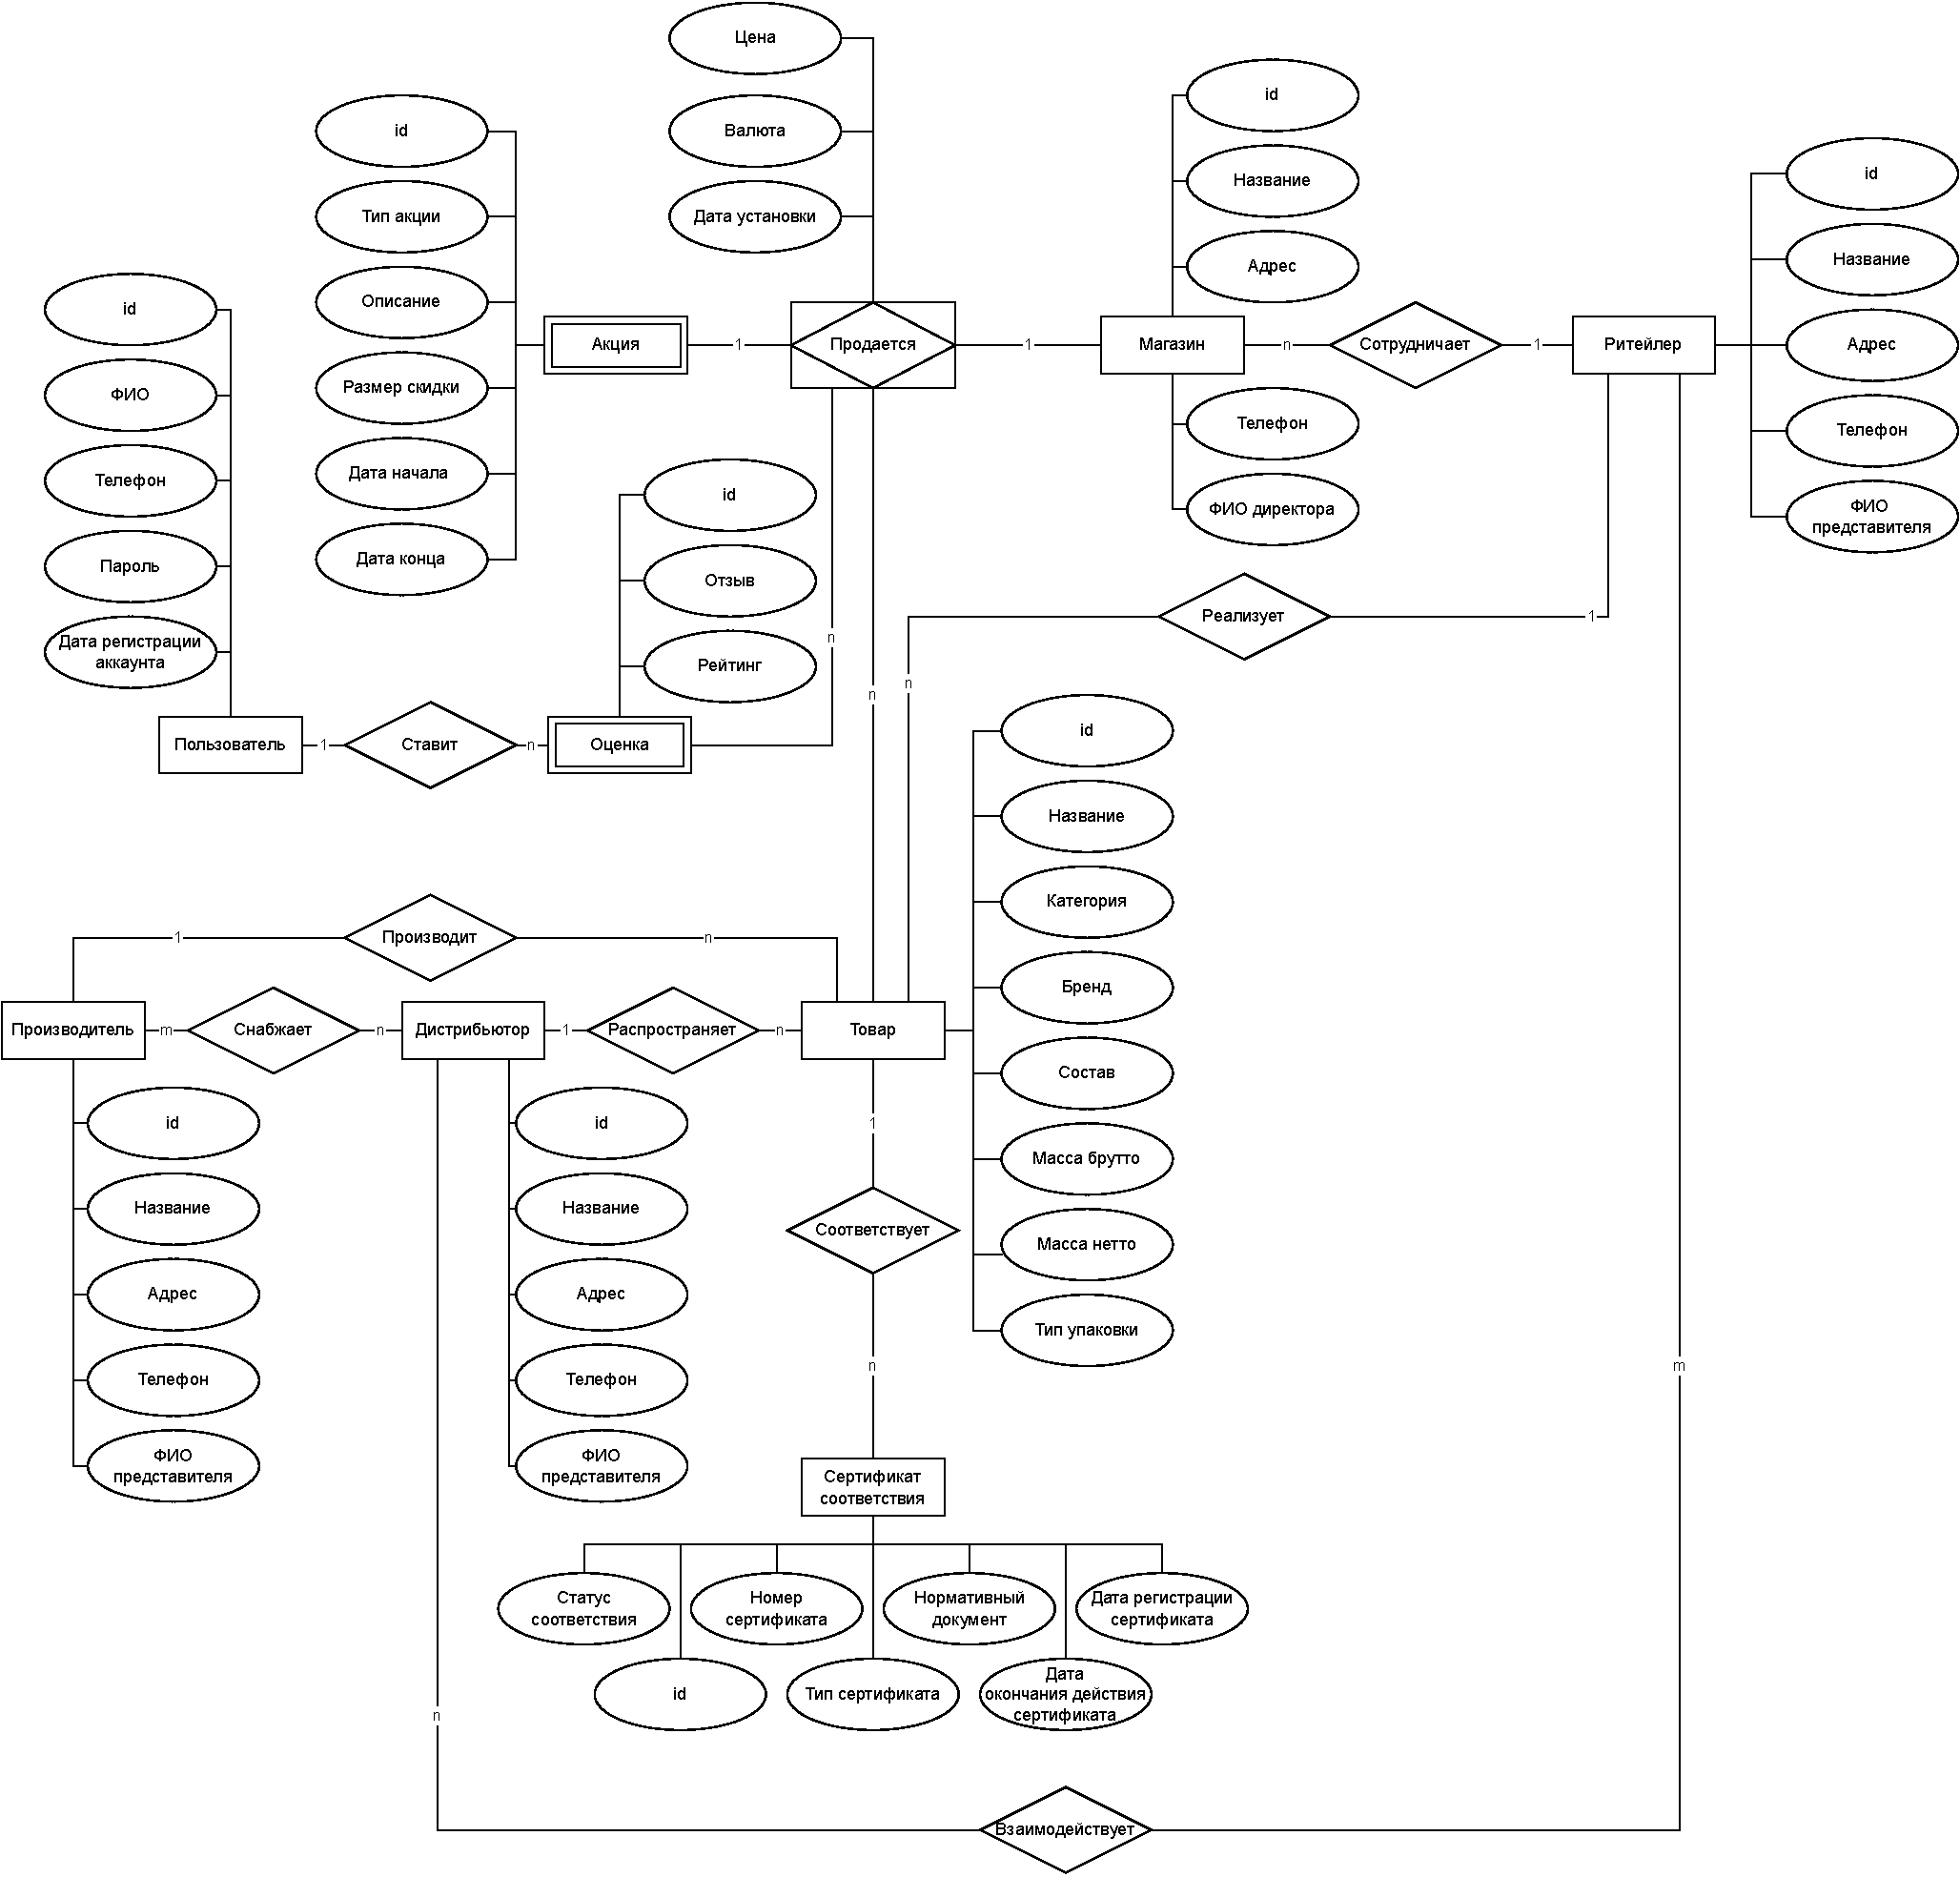
\includepdf[pages=-,pagecommand={},width=\textwidth]{inc/img/er-diag.drawio.pdf}

%\includesvgimage
%{er-diag.drawio} % Имя файла без расширения (файл должен быть расположен в директории inc/img/)
%{f} % Обтекание (без обтекания)
%{h} % Положение рисунка (см. figure из пакета float)
%{1\textwidth} % Ширина рисунка
%{ER-диаграмма сущностей проектируемой базы данных в нотации Чена} % Подпись рисунка

\includepdfimage
{er-diag.drawio.pdf} % Имя файла без расширения (файл должен быть расположен в директории inc/img/)
{f} % Обтекание (без обтекания)
{h} % Положение рисунка (см. figure из пакета float)
{1\textwidth} % Ширина рисунка
{ER-диаграмма сущностей проектируемой базы данных в нотации Чена} % Подпись рисунка

%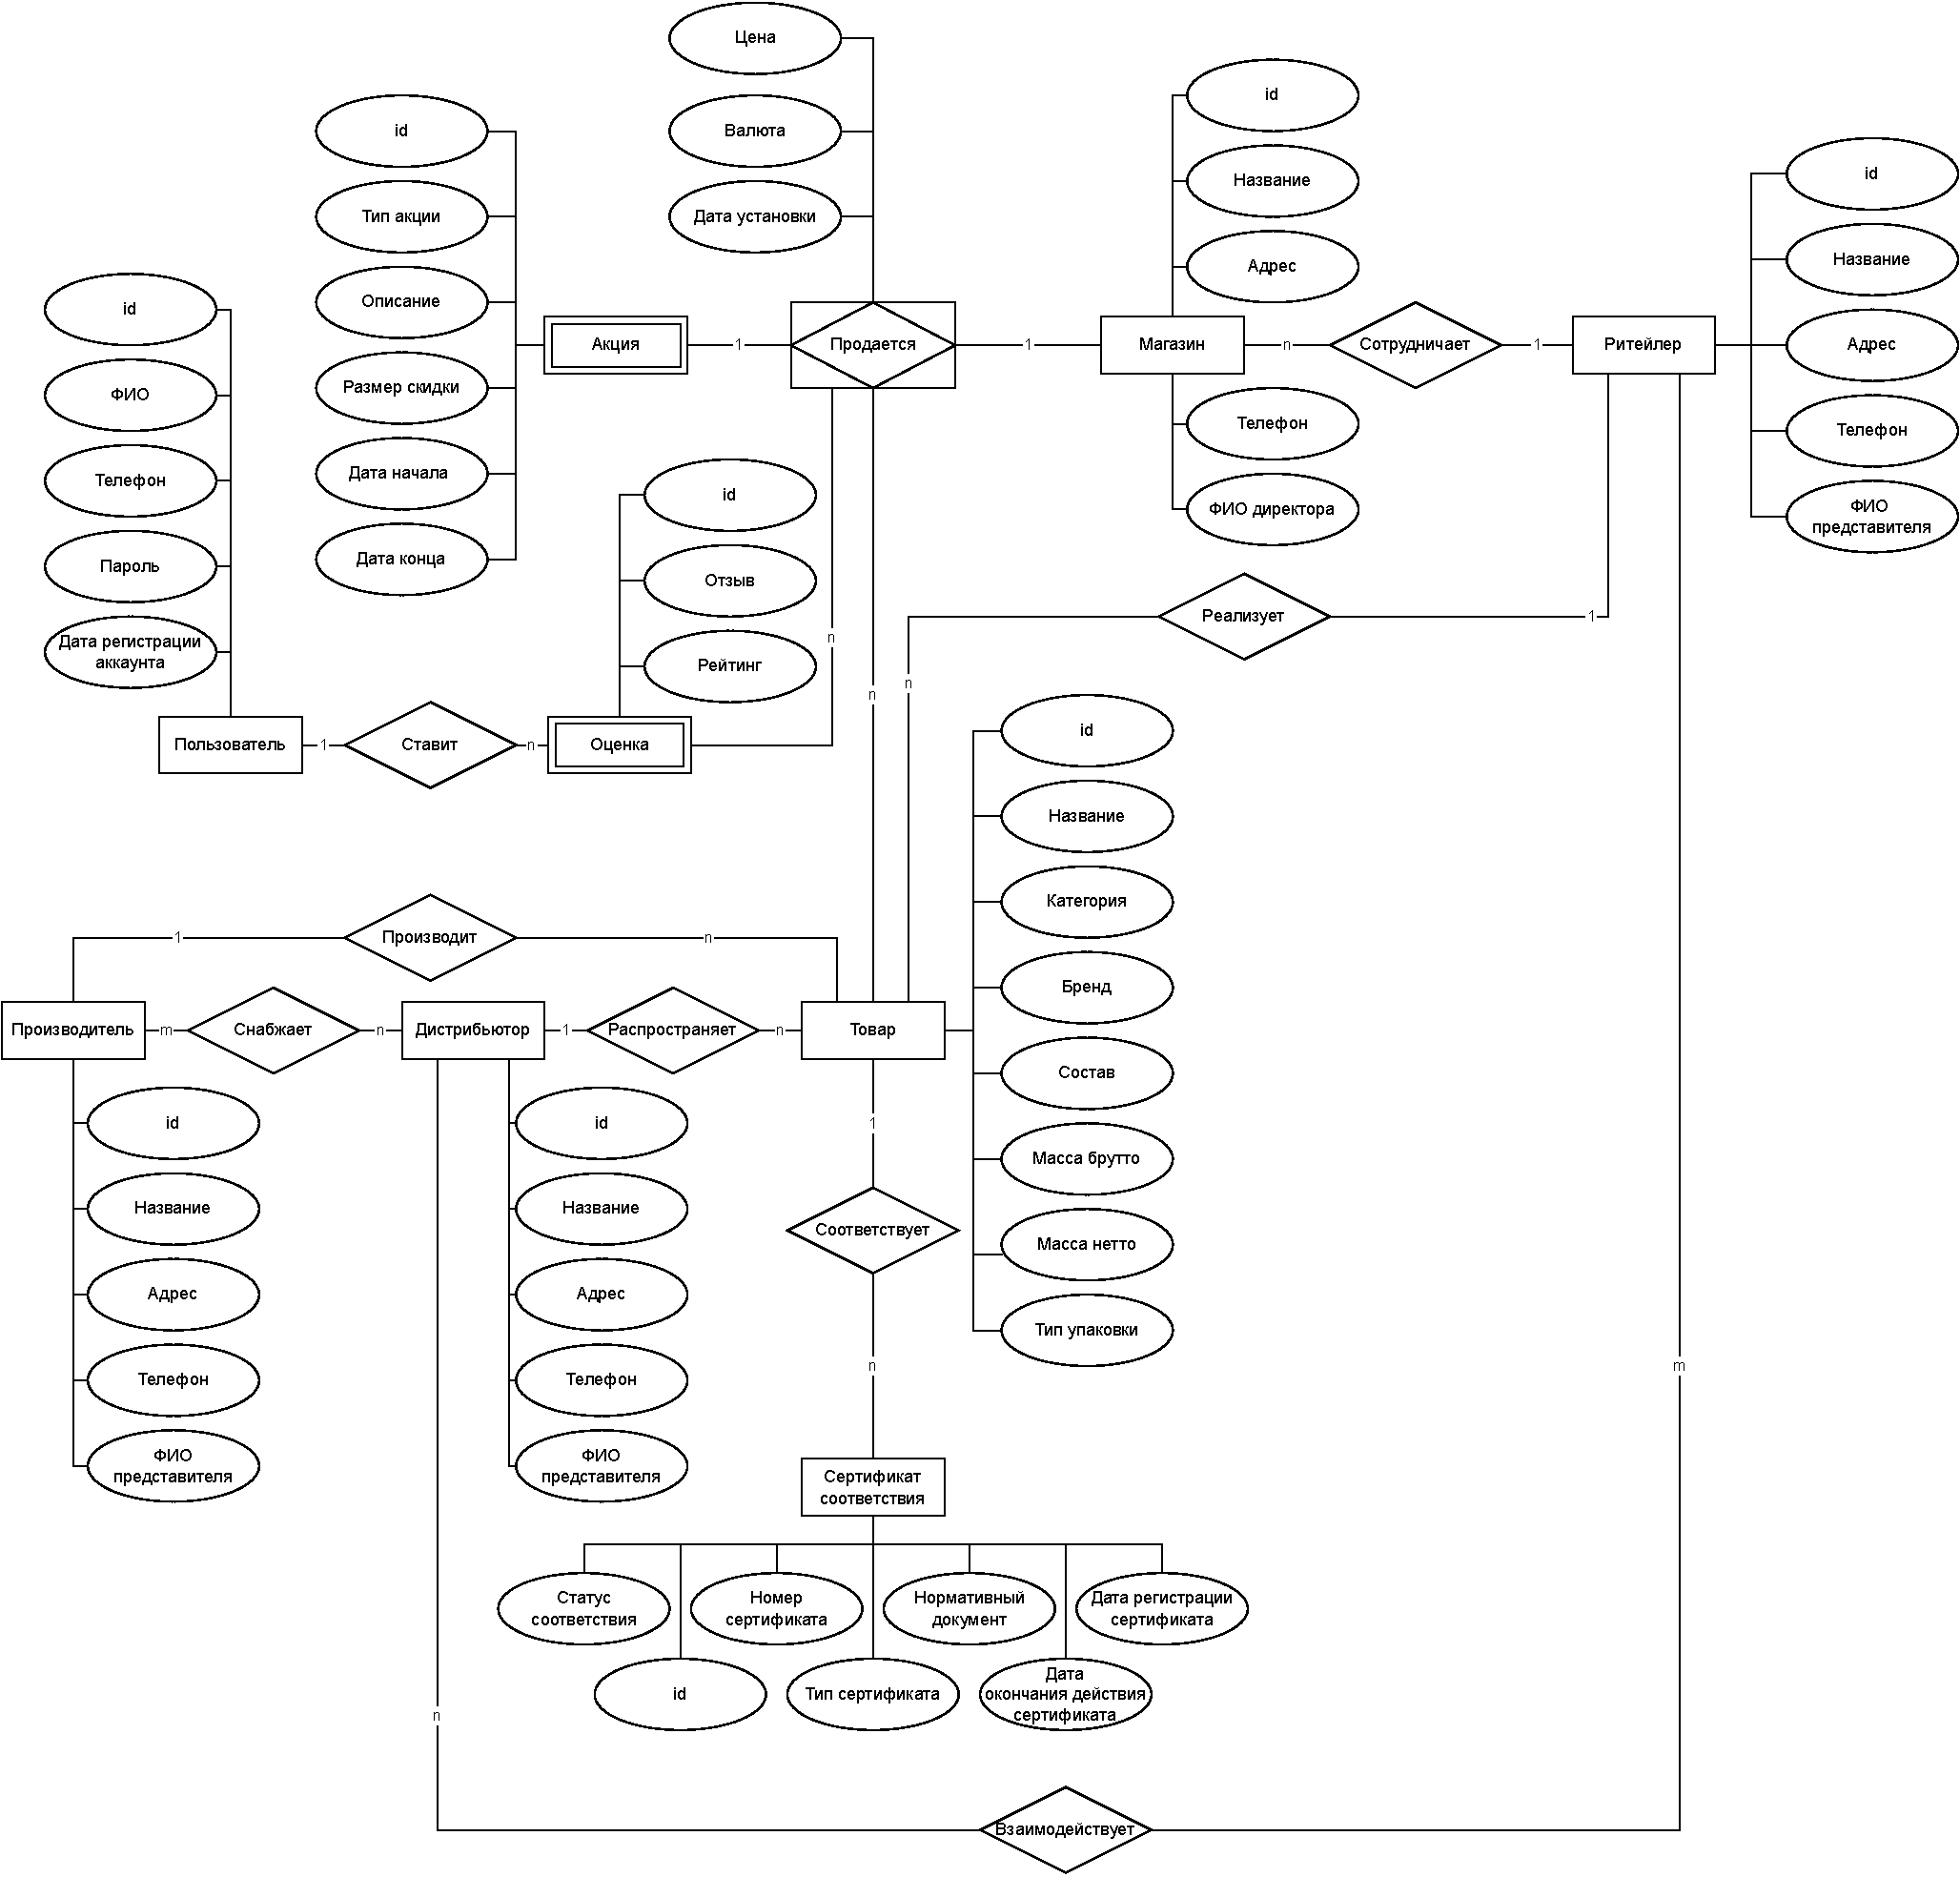
\includegraphics[width=\textwidth]{inc/img/er-diag.drawio.pdf}

\clearpage

\section{Формализация и описание пользователей проектируемого приложения к базе данных}

В соответствии выделенными в разрабатываемой базе данных сущностями выделяется 3 типа пользователей:

\begin{table}[ht]
	\begin{center}
		\begin{threeparttable}
			\caption{Типы пользователей и их описание}
			\label{tbl:db_roles}
			\begin{tabular}{|p{4.5cm}|p{10cm}|}
					\hline
					\textbf{Тип пользователя} & \textbf{Описание} \\ \hline
					Гость & Может просматривать всю информацию о товарах, сравнивать цены. \\
					\hline
					Зарегистрированный пользователь & Может все то же, что и гость, а также ставить оценки на товары, добавлять новые товары, вносить изменения в цену товара, а также добавлять новые магазины. \\
					\hline
					Администратор & Управляет всей системой. Может все то же, что и гость, а также удалять магазины, добавлять/удалять сертификаты на товары. \\ 
					\hline
				\end{tabular}
		\end{threeparttable}
	\end{center}
\end{table}

\clearpage

На рисунке \ref{img:use-case-diag.drawio.pdf} представлены диаграммы вариантов использования для различных пользователей системы:

\includepdfimage
{use-case-diag.drawio.pdf} % Имя файла без расширения (файл должен быть расположен в директории inc/img/)
{f} % Обтекание (без обтекания)
{h} % Положение рисунка (см. figure из пакета float)
{0.8\textwidth} % Ширина рисунка
{Диаграмма вариантов использования для различных пользователей системы} % Подпись рисунка

\clearpage

\section{Классификация и выбор СУБД по модели данных}

СУБД --- приложение, обеспечивающее создание, хранение, обновление и поиск информации в базах данных.

Модель данных --- это абстрактное и логическое определение объектов и его поведение, в совокупности составляющих доступ к данным, с которой взаимодействует пользователь~\cite{info_intro_db_williams}. С помощью модели данных могут быть представлены объекты предметной области и взаимосвязи между ними.

По модели данных СУБД разделяются на:

\begin{enumerate}
	\item дореляционные модели, которые, в свою очередь, делятся на:
	\begin{itemize}
		\item инвертированные списки;
		\item иерархические;
		\item сетевые.
	\end{itemize}
	\item реляционные модели данных;
	\item постреляционные модели данных.
\end{enumerate}

\subsection{Дореляционные базы данных}

Дореляционные БД подразделяются на инвертированные списки, иерархические БД и сетевые БД.

БД на основе инвертированных списков состоит из двух областей: основная и индексная области. Основная область представляет собой наборы файлов с записями. Записи в файле имеют фиксированную длину и расположены либо в произвольном порядке, либо упорядочены в соответствии с физической организацией хранения данных. Индексная область представляет собой индексные файлы -- файлы, содержащие значения ключей поиска и соответствующие этим значениям номера записей из файлов основной области \cite{info_inverted_lists}. В такой системе отсутствуют механизмы поддержания целостности хранимых данных, эта работа возлагается на программу, которая работает с такой БД.

Иерархическая БД состоих из трех основных элементов: физическая база данных, сегмент и поле. Поле представляет собой минимальную, неделимую единицу данных. Сегмент -- запись в базе данных, состоящая из полей. Для идентификации отдельного сегмента используется некоторый набор ключевых полей. В такой модели сегменты образуют ациклический древовидный граф, называемый физической базой данных. Физическая база данных должна удовлетворять следующим ограничениям \cite{info_inverted_lists}: 

\begin{itemize}[label*=--]
	\item в каждой физической БД должен существовать только один корневой сегмент;
	\item сегмент-предок может быть связан с произвольным числом сегментов-потомков;
	\item сегмент-потомок может быть связан только с одним сегментом-предком.
\end{itemize}

Благодаря данным ограничениям осуществляется поддержка ссылочной целостности между сегментами-предками и сегментами-потомками, однако нет поддержки целостности данных между сегментами, не входящими в одну иерархию.

Сетевая модель БД есть расширение иерархической: в иерархических структурах запись-потомок должна иметь в точности одного предка; в сетевой структуре данных потомок может иметь любое число предков\cite{info_db_kuznecov}. Основные термины сетевой модели баз данных включают элемент (узел) и связь. Узел представляет собой набор атрибутов, описывающих определённый объект. Сетевые базы данных можно визуализировать в виде графа. Логика извлечения данных в сетевой БД зависит от их физической организации, что делает эту модель не полностью независимой от приложения. Иными словами, при необходимости изменения структуры данных потребуется также внести коррективы в само приложение \cite{info_lections_db}. 

Преимущество дореляционных БД состоит в том, что они позволяют управлять данными на низком уровне. Недостатком является необходимость знания физической организации данных и зависимость прикладных систем от этой организации \cite{info_db_kuznecov}.

\clearpage 

\subsection{Реляционные базы данных}

Реляционная модель состоит из следующих трех частей: 

\begin{enumerate}[label={\arabic*)}]
	\item структурная --- описывает, из каких объектов состоит реляционная модель. Определяется, что единственной структурой данных, используемой в реляционных БД, являются нормализованное n-арное отношение \cite{info_db_kuznecov};
	\item целостная --- отношения должны удовлетворять определенным условиям целостности \cite{info_lections_db}:
	\begin{itemize}[label*=--]
		\item целостность сущности -- любой кортеж любого отношения должен отличаться от любого другого кортежа этого же отношения;
		\item ссылочная целостность -- для каждого значения внешнего ключа, присутствующего в дочернем отношении, в родительском отношении должен существовать кортеж с соответствующим значением первичного ключа.
	\end{itemize}
	\item манипуляционная \cite{info_lections_db} --- манипулирования отношениями осуществляется средствами реляционной алгебры и/или реляционного исчисления.
\end{enumerate}

Основными достоинствами реляционных БД является наличие небольшого набора абстракций, простого и в то же время мощного математического аппарата, возможность ненавигационного манипулирования данными без необходимости знания конкретной физической организации баз данных во внешней памяти \cite{info_db_kuznecov}.

\subsection{Постреляционные базы данных}

Постреляционная модель в общем случае есть расширение классической реляционной модели. В такой модели используются структуры, позволяющие хранить в полях таблицы другие таблицы, а в качестве языка запросов используется расширенный SQL \cite{info_post_db}.

Преимуществом такой модели данных является возможность представления связанных реляционных таблиц одной постреляционной таблицей, что расширяет возможности описания сложных предметов реального мира, а недостатком -- сложность в обеспечении целостности данных \cite{info_db_sopchenko}.
                         
\section*{Вывод} 


\begin{table}[ht]
	\begin{center}
		\begin{threeparttable}
			\caption{Сравнение баз данных по модели данных}
			\label{tbl:cmpDbByDataModel}
			\begin{tabular}{|c|c|c|c|}
				\hline
				Модель данных & \makecell{Обеспечение \\ целостности \\ сущностей} & \makecell{Обеспечение \\ ссылочной \\ целостности} & \makecell{Независимость \\ от физической \\ организации \\ данных} \\
				\hline
				\makecell{Дореляционная} & + & + & -  \\
				\hline
				\makecell{Реляционная} & + & + & + \\
				\hline
				\makecell{Постреляционная} & - & + & + \\
				\hline
			\end{tabular}
		\end{threeparttable}			
	\end{center}
\end{table}


В данном разделе была проанализирована предметная область, рассмотрены существующие решения. На основе анализа предметной области была формализована задача и данные, описаны типы пользователей. 

Для разрабатываемой базы данных необходимо обеспечение целостности сущностей, целостных связей между сущностями, а также независимость от физической организации данных. Дореляционные модели данных не подходят, поскольку они зависимы от физической организации хранения данных, а в моделях на основе инвертированных списков отсутствуют ограничения целостности. Не подходит также и постреляционная модель, поскольку в этой модели возникают сложности с обеспечением целостного хранения данных из-за отмены ограничения на атомарность значений атрибутов. Таким образом, согласно с таблицей \ref{tbl:cmpDbByDataModel}, для хранения данных была выбрана реляционная модель, поскольку она удовлетворяет всем необходимым требованиям.